[Youtub] https://www.youtube.com/watch?v=Z9dvM7qgN9s\&t=446s


[출처] /Users/leejaekun/.gitconfig
1.VS Code를 Git diff tool

1. 명령어중에 code --help를 실행하면 도움말이 표시되는지 확인 합니다.\\
표시되지 않는다면 \\
macOS: Command Palette에서 Shell Command: Install ‘Code’ command in path를 선택합니다.\\
윈도우즈: VS Code 를 설치하는 동안 PATH 에 추가하기를 선택합니다.\\
리눅스: .deb 또는 .rpm 패키지를 사용하여 설치합니다.\\

\noindent > git config --global core.editor "code --wait"\\
에디터를 visual studio code 로 설정하고, code를 닫기 전까지 응답하지 않음. \\

\noindent > git config --global core.autocrlf true  (window user 의 경우 )\\
\noindent > git config --global core.autocrlf input (mac user 의 경우 )\\
%
\begin{figure} [!htbp] % [!htbp] 
	\centering
	\captionsetup{justification=centering,margin=1cm}
	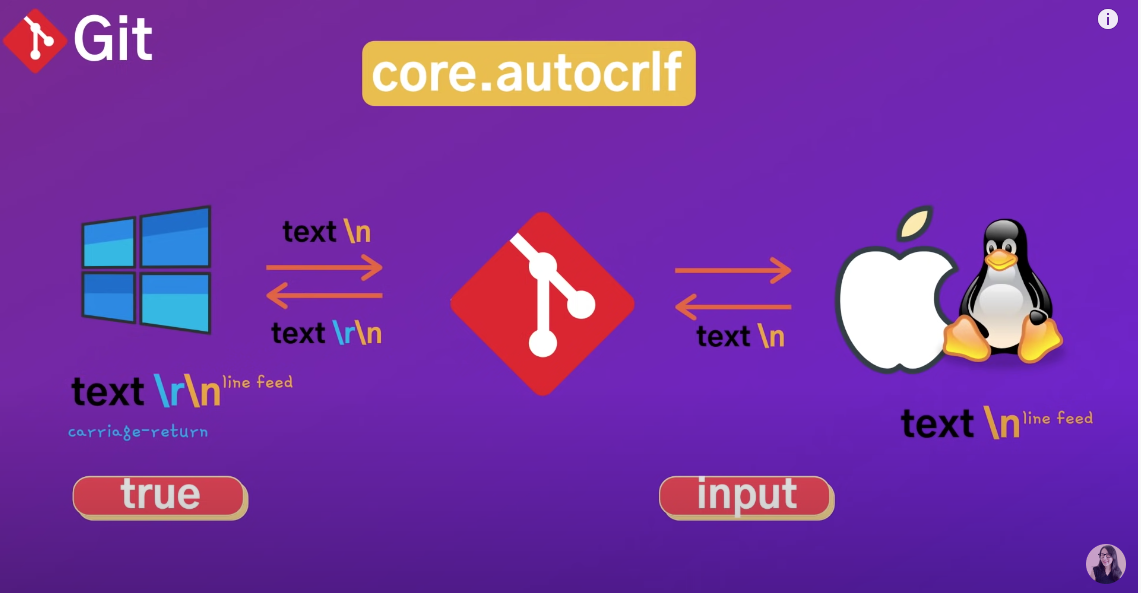
\includegraphics[width=0.7\linewidth]{./fig/autocrlf.png}
	\caption{window / max의 캐리지리턴}
	\label{fig:autocrlf}
\end{figure} 
%




\newpage
\setstretch{1.6} 
\noindent [출처] \href{https://reddb.tistory.com/146?category=948284}{\color{blue}{https://reddb.tistory.com/146?category=948284}}

\noindent \textbf{git init} : 초기화. .git 폴더가 만들어 진다.\\
%
\textbf{git status} : git 의 상태를 출력 합니다.\\
%
\begin{itemize}
	\item On branch master : 현재 마스터 브랜치가 존재
	\item No commits yet : 아직 커밋한 파일이 없음 
	\item nothing to commit : 현재 커밋할 파일이 없음.
\end{itemize}
%
\begin{figure} [!htbp] % [!htbp] 
	\centering
	\captionsetup{justification=centering,margin=1cm}
	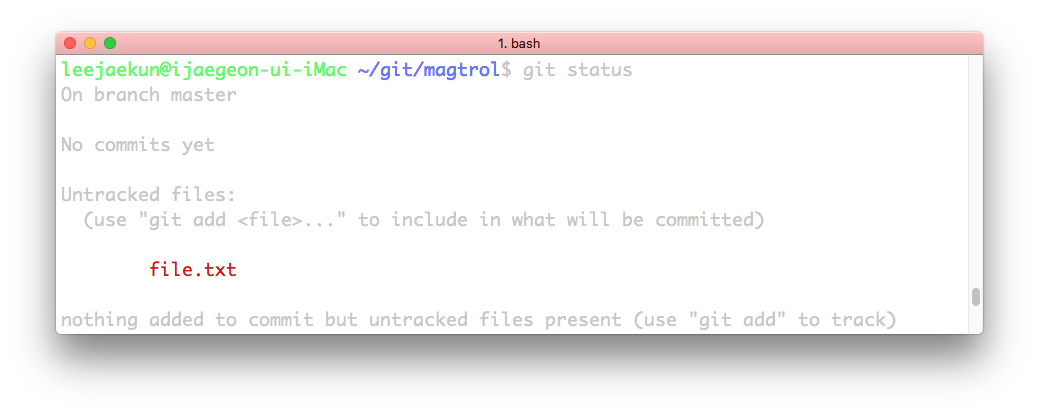
\includegraphics[width=0.7\linewidth]{./fig/status.png}
	\caption{git status 예제}
	\label{fig:status}
\end{figure} 
%
파일을 생성을 하고 git status를 입력을 하면 Untracked files 하는 변화된 내용이 출력됩니다.
깃에서 버젼관리를 하지 않는 파일들을 Untracked files 라고 합니다.\\
%
\textbf{git add} : 파일을 스테이지로 올립니다.
%
\begin{figure} [!htbp] % [!htbp] 
	\centering
	\captionsetup{justification=centering,margin=1cm}
	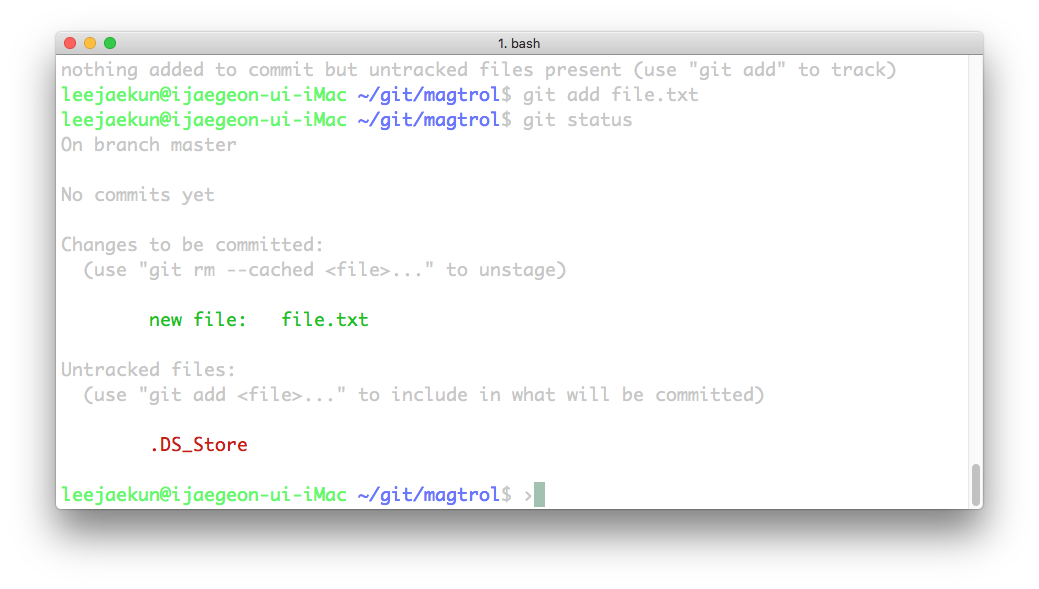
\includegraphics[width=0.7\linewidth]{./fig/add.png}
	\caption{git add 예제}
	\label{fig:add}
\end{figure} 
%
git status 를 입력하면 Change to be commited 라는 변화된 내용으로 출력 됩니다.
이는 파일이 커밋할 준비가 되었다는 상태입니다. \\
%
\noindent \textbf{git commit} : 파일을 커밋합니다. \\
그림\ref{fig:commit}\과 같이 git commit -m "넣고 싶은 메시지" 형태로 입력을 합니다. \\
%
\begin{figure} [!htbp] % [!htbp] 
	\centering
	\captionsetup{justification=centering,margin=1cm}
	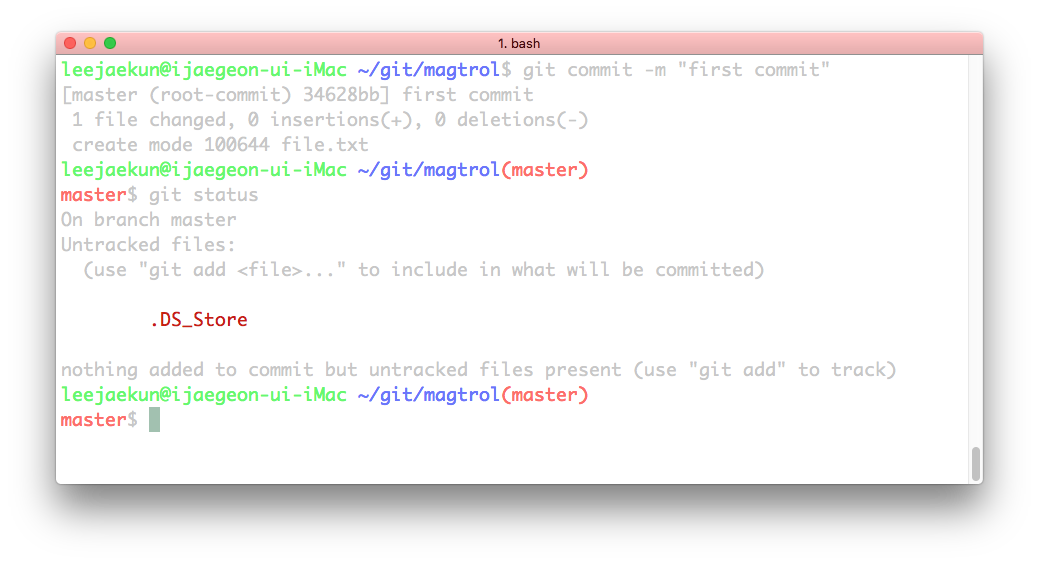
\includegraphics[width=0.7\linewidth]{./fig/commit.png}
	\caption{git commit 예제}
	\label{fig:commit}
\end{figure} 
%
 \textbf{git log} : commit 되어 있는 상태를 보여준다. \\
 내가 입력한 메시지(수정내용 요약) 내용을 포함한다. \\
 %
\begin{figure} [!htbp] % [!htbp] 
	\centering
	\captionsetup{justification=centering,margin=1cm}
	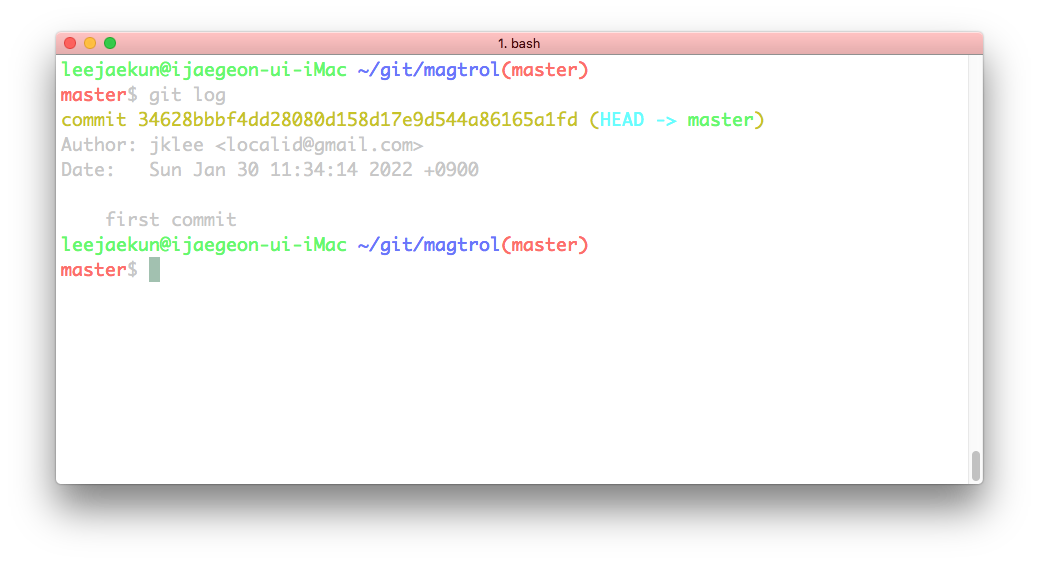
\includegraphics[width=0.7\linewidth]{./fig/log.png}
	\caption{git log 예제}
	\label{fig:log}
\end{figure} 
%
 
 \newpage
 \noindent \large{\href{https://gist.github.com/480/4681b67d2a906db8c6c1321cc678f05f}{\textbf{\color{blue}깃 리모트 변경 하기}} }\\
\newline \normalsize
% 
\textbf{기존 리포지토리 깔끔하게 pull / push} \\
git pull \\
git add . \\
git commit -m "clean push" \\
git push \\
%
\newline
\textbf{기존 리포지토리 remote 제거} \\
git remote remove origin \\
%
\newline
\textbf{새 리포지토리 remote 추가} \\
git remote add origin https://github.com/계정/리포지토리 \\

 \newpage
 \noindent \href{https://www.yalco.kr/lectures/git-github/}\textbf{\color{blue}{얄코 강좌}} \\
 iTerms2 설치와 터미널 셋팅 \\
 %
\begin{figure} [!htbp] % [!htbp] 
	\centering
	\captionsetup{justification=centering,margin=0.5cm}
	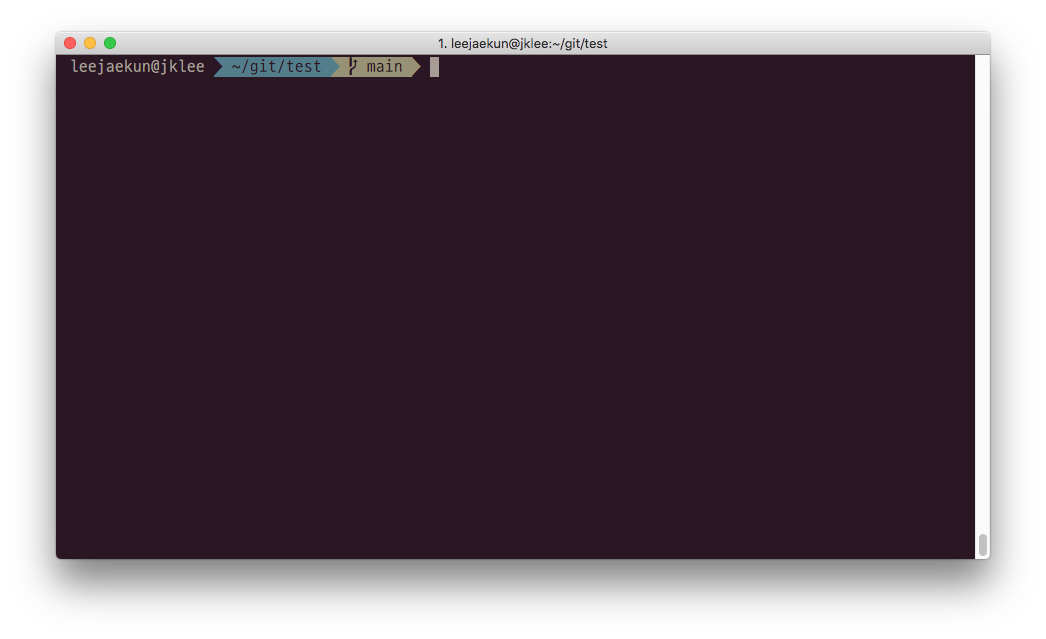
\includegraphics[width=0.7\linewidth]{./fig/zsh-iTerms2.png}
	\caption{zsh 설치 후, iTerms2 화면 예제}
	\label{fig:iTerms2}
\end{figure} 
%
 
 
 
